\documentclass[conference]{IEEEtran}
    

\usepackage{graphicx,times,amsmath}

% Correct bad hyphenation here
\hyphenation{op-tical net-works semi-conduc-tor IEEEtran}

\IEEEoverridecommandlockouts        

\textwidth 178mm
\textheight 239mm
\oddsidemargin -7mm
\evensidemargin -7mm
\topmargin -6mm 
\columnsep 5mm

\begin{document}

% Paper title: keep the \ \\ \LARGE\bf in it to leave enough margin.
\title{\ \\ \LARGE\bf Reactiveness and Navigation in Computer Games:\\ Different Needs, Different Approaches \thanks{Diego Perez is an independent author, email: {\tt Diego.Perez.Liebana@gmail.com}; Miguel Nicolau, Michael O'Neill and Anthony Brabazon are with the Natural Computing Research and Applications Group, University College Dublin, Ireland, email {\tt Miguel.Nicolau@ucd.ie}, {\tt Michael.ONeill@ucd.ie}, {\tt Anthony.Brabazon@ucd.ie}}}


\author{Diego Perez, Miguel Nicolau, Michael O'Neill and Anthony Brabazon}


\maketitle

\begin{abstract}
This paper presents an approach to the Mario AI Benchmark problem, using
the A* algorithm for navigation, and an evolutionary process combining
routines for the reactiveness of the resulting bot. The Grammatical
Evolution system was used to evolve Behaviour Trees, combining both types of
routines, while the highly dynamic nature of the environment required specific
approaches to deal with over-fitting issues. The results obtained highlight
the need for specific algorithms for the different aspects of controlling a bot
in a game environment, while Behaviour Trees provided the perfect
representation to combine all those algorithms.
\end{abstract}

%%%%%%%%%%%%%%%%%%%%%%%%%%%%%%%%%%%%%%%%%%%%%%%%%%%%%%%%%%%%%%%%%%%%%%%%%%%%%%%
\section{Introduction} \label{sec:intro}
%%%%%%%%%%%%%%%%%%%%%%%%%%%%%%%%%%%%%%%%%%%%%%%%%%%%%%%%%%%%%%%%%%%%%%%%%%%%%%%

Computer games can be an extremely challenging benchmark for Evolutionary
Algorithms, and for Artificial Intelligence in general. The challenges
presented go from static or dynamic path planning and single move optimisation, to
adaptation in dynamic environments, learning and cooperative behaviours. Extra
challenges include the need for human-like behaviours, avoidance of
repetitiveness, and conformity to the ability of human-opponents.

Evolutionary algorithms can help to solve some of these problems, making them
particularly suitable for certain game environments. Their stochastic nature,
along with tunable high- or low-level representations, contribute to the
discovery of non-obvious solutions, while their population-based nature can
contribute to adaptability, especially in dynamic environments. There are
also drawbacks, however: traditionally, the games industry tends to adopt
traditional, \textit{classic AI} algorithms, such as \textit{A*},
%\textit{min-max} and others, because many game industry developers are 
%more used to work with these algorithms.
\textit{min-max} and others, due to their field-tested reliability, versus the
stochastic, variable nature of evolutionary algorithms.

The main objective of this paper is to investigate the applicability of Genetic
Programming \cite{Koz92} (GP) systems to evolve Behaviour Trees \cite{CH07}
%(BTs) in order to obtain a better reactiveness to dynamic game environments. 
(BTs), in order to improve the reactiveness of agents in dynamic game environments. 

Behaviour Trees (BTs) were introduced as a way to encode
%formal system specifications \cite{Dro04,CH07}. Recently, they have been
formal system specifications \cite{CH07}. Recently, they have also been
used to encode game AI in a modular, scalable and reusable
manner \cite{CDC10}. They have been used in high-revenue commercial games, such
as \textit{Halo} \cite{Isl05} and \textit{Spore} \cite{Mch07}, smaller indie games, such
as \textit{Fa\c{c}ade} \cite{MS04}, and many other unpublished uses
\cite{CDC10}, which illustrate their flexibility and growing importance in the
commercial game AI world.

The Mario AI Benchmark~\cite{TKK09} was used, as it provides this kind of environment, with
a series of obstacles to bypass, all the while avoiding (or eliminating)
enemies and collecting bonuses as coins or items. The reactive nature of BTs can 
%be seen as a powerful representation for a dynamic environment, and the flexibility 
be used as a powerful representation for dynamic environments, and the flexibility 
%provided by Grammatical Evolution \cite{OR03} (GE) facilitates the behaviour tree 
%evolution and evaluation in a live play scenario.
provided by Grammatical Evolution \cite{OR03} (GE) facilitates the evolution of
behaviour tree structures, and their evaluation in a live play scenario.

% THIS IS COMPETITION!
%%The best evolved bot was sent to the 2010 Mario AI competition \cite{MAI10}.
%%This is a contest organized by Julian Togelius and Sergey Karakovskiy, 
%%and it is the successor to the competition held by the same organizers 
%%in 2009 \cite{JSR10}. The 2010 competition took place in four different 
%%events: EvoStar 2010, World Congress on Computational Intelligence 
%%(WCCI) 2010, Conference on Computational Intelligence and Games
%%(CIG) 2010 and Games Innovation Conference (GIC) 2010.
%
%%The participants of the competition are requested to submit a bot that can
%%participate in up to three different tracks: gameplay, learning and level
%%generation. The bot presented by the authors for this competition took part in
%%the gameplay track of CIG-2010, where the bots are evaluated in levels that
%%have not been seen previously by the competitors. 
%
%The best evolved bot was sent to the gameplay track of the 2010 Mario AI
%competition \cite{TKB10}, where the bots are required to navigate through
%unseen levels. The results obtained show the viability of the technique
%presented; pitted against fierce competition, it reached fourth place, very
%close to the top three.
%

%Another challenge also faced in this paper is the compatibility of two
%different approaches to solve the navigation of the bot through the levels. On
%one hand, Mario has to deal with enemies and other dynamic objects that can
%hurt him or power him up, so there is a need of a reactive management. 
%On the other hand, Mario has to advance in the level in order to reach its end, 
%dealing with structural hazards that make some kind of path planning necessary. 
%The BTs, driven by evolution, take care of the reactive part of the behaviour
%while the higher level navigation is managed by an A* implementation.
One of the major challenges faced in this environment is the
combination of navigation and reactiveness, in order to achieve the ultimate
goal (reach the end of each level). On one hand, Mario has to deal with
enemies and other dynamic objects that can hurt him or power him up, so there
is the need of instant, reactive behaviour. On the other hand, Mario has to
advance through the level in order to reach its end, dealing with structural
hazards (jumps, traps, etc.), that require some kind of path planning.
The approach described here uses an A* implementation to dynamically
devise a path through each level, while BTs, driven by evolution, are
responsible for the reactive behaviour of the agent.

This paper starts by giving some literature background. The Mario AI Benchmark
environment is then described, followed by an overview of the path finding
algorithm used for navigation. An introduction to Behaviour Trees follows, detailing
their specific application to the problem; this is followed by a section
detailing the application of the Grammatical Evolution system.
Finally, the experimental setup and results obtained are discussed.

%%%%%%%%%%%%%%%%%%%%%%%%%%%%%%%%%%%%%%%%%%%%%%%%%%%%%%%%%%%%%%%%%%%%%%%%%%%%%%%
\section{Relevant Literature}
%%%%%%%%%%%%%%%%%%%%%%%%%%%%%%%%%%%%%%%%%%%%%%%%%%%%%%%%%%%%%%%%%%%%%%%%%%%%%%%

The literature provides us with some examples of using evolutionary
computation algorithms to control AI agents in game environments. In terms 
of anticipating and reactive behaviour, examples include the work of Nason and
Laird \cite{NL04}, who proposed an approach to add anticipation to bots in the
\textit{Quake} game, using reinforcement learning; and that of Thurau et
al.~\cite{TBS04}, who produced agents that try to learn desirable behaviour
based on imitation of already existing players, by training a neural network on data
gained from human players. Mora et al.~\cite{MMM10} used a Genetic Algorithm 
to fine-tune parameters of an existing AI bot code, and Genetic Programming to 
change the default set of rules or states that define a behaviour; and finally, 
Priesterjahn\cite{Pri09} used Evolution Strategies to evolve bot players in the 
\textit{Quake III} game, by using an evolutionary process to create and select 
input/output rules, with inputs being a grid representation of the world 
around the bot, along with an associated action.

%The work of Lim et al.~\cite{LBC10} is the only one that specifically
%deals with evolving behaviour tree structures.  It used GP
%to evolve AI controllers for the ``DEFCON'' game. It
%starts with a set of hand-designed trees, encoding feasible behaviours for each
%of the game's five parts; separate GP executions are then performed for
%each part, creating new behaviours from the original set. The final combined
%tree, after evolution, was pitted against the standard AI controller that comes
%with the game, and achieved a success rate superior to $50\%$. Some hurdles
%were encountered in this work, such as how to deal with the exchange of typed
%tree structures between individuals; these, amongst others, are easily dealt
%with by using grammar-based GP systems, such as GE, presented next.

The work of Lim et al.~\cite{LBC10} specifically
dealt with evolving behaviour tree structures. It used GP
to evolve AI controllers for the \textit{DEFCON} game; the final evolved
tree was pitted against the standard DEFCON AI controller, and achieved a
success rate superior to $50\%$. Some hurdles
were encountered in this work, such as how to deal with the exchange of typed
tree structures between individuals; these, amongst others, are easily dealt
with by using grammar-based GP systems. An earlier version of the work
described in the current paper highlighted that \cite{PNO11}: the Grammatical
Evolution system was applied to the Mario AI Benchmark, evolving Behaviour
Tree controllers.

The literature is also broad in terms of using path planning for navigation, 
both in robotics~\cite{MF03} and in games, such as \textit{Unreal
Tournament}, \textit{Quake III} or \textit{Half Life}~\cite{Bir99}. The most
common algorithm used for path finding is A*, because of its great performance,
accuracy and efficiency~\cite{BT98}. 

In the Computational Intelligence and Games 
(CIG) 2009 conference, the three top entries for the Mario AI Championship, 
by Robin Baumgarten, Peter Lawford and Andy Sloane~\cite{TKB10}, used 
an A* algorithm to manage local navigation. Additionally, the CIG 2010 Mario 
AI Championship was won by Slawomir Bojarski~\cite{BC10}, who also 
implemented an A* to determine keystrokes for high level actions. 

Furthermore, path planning algorithms are usually combined with other reactive 
behaviours or systems, such as general planning, obstacle avoidance, 
speech or 3D animation~\cite{CBP99}. 


%%%%%%%%%%%%%%%%%%%%%%%%%%%%%%%%%%%%%%%%%%%%%%%%%%%%%%%%%%%%%%%%%%%%%%%%%%%%%%%
\section{The Mario AI Benchmark} \label{sec:marioBench}
%%%%%%%%%%%%%%%%%%%%%%%%%%%%%%%%%%%%%%%%%%%%%%%%%%%%%%%%%%%%%%%%%%%%%%%%%%%%%%%

The Mario AI Benchmark was used for the experiments
described in this paper. This benchmark is an open source 
software, developed by Togelius et al.~\cite{TKK09}, and it was used 
in the 2010 Mario AI competitions.
It allows the creation of agents that play the game, by 
providing two methods: one to retrieve and process environment information,
and the other to specify the actions of the bot.

%%%%%%%%%%%%%%%%%
\subsection{Environment information} \label{subsec:marioBenchEnviron}

All the information that can be used to analyse the world around Mario is given
in two matrices (21x21). Each of these provides 
data about the geometry of the level, and the enemies that populate it.
These arrays are centred around Mario, so 10 grid cells in each direction from the
position of Mario can be processed every cycle (see Fig.~\ref{fig:matrix}).

\begin{figure} [ht]
	\begin{center}
	\includegraphics[scale=0.45]{images/trapMatrix}
	\caption{Matrix centred in Mario.}
	\label{fig:matrix}
	\end{center}
\end{figure}

%Additionally, three different levels of detail can be specified to retrieve data
%in both arrays, depending on the information we are looking for:
%\begin{itemize}
%\item \textbf{Zoom 2:} The data is represented in a binary array. For enemies, 
%0 means that there is no enemy on that position, while 1 means there is some
%enemy. Likewise, for the level scene, 1 means that there is an obstacle and 0
%that Mario can pass through.
%\item \textbf{Zoom 1:} This zoom levels represents the data with an integer, 
%gathering groups of objects with a common identifier. For the enemy information, 
%0 means no enemy at all, 2 represents an enemy that can be killed by Mario by
%jumping on it and 9 it is set for those enemies that can be killed just shooting at them. 
%For the level scene, different identifiers represent types of blocks, like those
%that can or can not be broken, contain hidden items or can spawn enemies.
%\item \textbf{Zoom 0:} This zoom level is a very close view of the internal 
%representation of the engine, where every kind of enemy or block in the 
%level has its own identifier, different from any other entity in the game.
%\end{itemize}


Additionally, three different levels of detail can be specified to retrieve data
in both arrays, depending on the information we are looking for. \textbf{Zoom 0}
represents the world with a different integer for each entity in the game, whereas
\textbf{Zoom 2} gives the simplest possible representation, 1 meaning enemy (or
obstacle) presence and 0 absence of it. As a mid term, \textbf{Zoom 1} categorizes
the information in useful groups, such as enemies that can be killed by
stomping, those that can be killed by shooting, different types of blocks, etc.

Apart from this information, more useful input represents the
current state of the game. The Mario \textbf{position} is a pair of
values that indicates the coordinates in pixels of Mario in the level. The
Mario \textbf{status} details the state of the game: running, win or dead. 
During the game, Mario can be small or big, with or without being able to fire, which
is represented by Mario's \textbf{mode}. There are also some Mario \textbf{state 
indicators}, that provide data such as the ability of Mario to shoot and jump, 
the time left for the level and whether Mario is on the ground or not.
Finally, some Mario \textbf{kill statistics} are also available, such as the number of enemies killed 
and how they died (by stomp, by fire or by shell bashing).

%%%%%%%%%%%%%%%%%
\subsection{Mario effectors} \label{subsec:marioBenchEffectors}

The actions that can be performed by Mario are all the different inputs that a
human player could use with a control pad. They are represented as a
boolean array, where each control has a concrete index assigned. 

%The controls to use are the directions (\textit{Left, Right, Up, Down}), the 
%\textit{Jump} control and a common button to \textit{Fire} and \textit{Jump}.  
%This last effector can used to make Mario to go faster, but it only works if he is 
%moving to the right or left. Jumps while pressing this button also make Mario
%reach farther platforms.

%The controls to use are the following:
%\begin{itemize}
%\item \textbf{Directions:} One different for each direction: Left, Right,
%Up and Down.
%\item \textbf{Jumping:} To make Mario jump.
%\item \textbf{Speed and Fire:} Mario can fire, if he is in the proper mode,
%by using this control. This input can also be used to make Mario to go faster, but it only 
%works if he is moving to the right or left. Jumps while pressing this button also 
%make Mario reach farther platforms.
%\end{itemize}

The controls that may be used are the directions (\textit{Left}, \textit{Right}, 
\textit{Up} and \textit{Down}), a button 
for jumping and a command to both fire and speed up. Going faster only 
works if Mario is moving to the right or left. Jumps while pressing this button also 
make Mario reach farther platforms.


%%%%%%%%%%%%%%%%%%%%%%%%%%%%%%%%%%%%%%%%%%%%%%%%%%%%%%%%%%%%%%%%%%%%%%%%%%%%%%%
\section{Deliberative vs. Reactive: A* for navigation}
%%%%%%%%%%%%%%%%%%%%%%%%%%%%%%%%%%%%%%%%%%%%%%%%%%%%%%%%%%%%%%%%%%%%%%%%%%%%%%%

The implementation proposed in this paper controls how Mario moves through the level
in two different points of view: reactive and deliberative (or path planning).

%%%%%%%%%%%%%%%%%%%%%%%%%
\subsection{Reactive behaviours}

Reactive behaviours are concerned with all the elements in the
game that can change their position. In this case, entities that move are enemies, 
such as evil mushrooms, bullets or flying turtles, which can follow different 
types of trajectories. Also included in this category are
items that can appear in the level after pushing brick blocks, like bonus mushrooms
(which make Mario big) and fire flowers (which give Mario the ability to shoot).

In this agent, the Grammatical Evolution algorithm is in charge of managing the
reaction to these entities, through the evolution of Behaviour Trees; these
systems and their combination are detailed in Sections \ref{BTs} and \ref{GE}.
%For this 
%to happen, several leaf nodes are provided order to give the GE the tools
%for detecting, chasing, avoiding and killing them, as stated in the section 
%\ref{subsec:bt4Mario}.


%%%%%%%%%%%%%%%%%%%%%%%%%
\subsection{Path planning with A*}

%In order to use A* for navigation, it is obvious that we need a graph
% to use in the level. The Mario Benchmark does not provide any graph, or
In order to use A* for navigation, a graphical representation of the level is
required. The Mario Benchmark does not provide any graph, or
%even a map, of the level that is being played. Furthermore, we also have
%to take into account that the level geometry can change during the game: 
even a map, of the level that is being played. Furthermore, the level geometry
can change during the game: 
Mario can break blocks and new paths are created. For this reason, 
the creation process of the map (and, hence, the graph) is executed frequently.
In this section, this map and graph creation process is explained in detail.

%--------------------------------------------
\paragraph{Building the map of the level}

The first problem that must be faced when dealing with path planning is 
the world representation. In the case of the Mario Benchmark, the agent has
no access to the map of the level, so it has to build one as Mario
is moving through it. The only way to examine the 
environment is to read the information available in the level matrices.

However, this information is relative to Mario's position (from now on, \textit{local
coordinates}), while the map of the level should be built in absolute values
(or \textit{world coordinates}). Furthermore, Mario's position is provided in pixels
with the origin at the upper left corner of the beginning of the level, whereas the 
local information matrix gives the information in grid cells units. For instance, Mario 
could be at (225, 53) while a brick block has been detected in (+1, -2).

Knowing that every cell block is equivalent to a 16x16 pixels square, we can 
easily translate the coordinates from local to world system. In the 
previous example, Mario would be in the coordinates $(225/16, 53/16) = 
(14,3)$, and the brick block in $(14+1, 3-2) = (15,1)$.

Using this conversion system, we can determine the position of every unit in the
level in a discrete grid. Fig.~\ref{fig:trap} shows a portion of a level, and 
Fig.~\ref{fig:trapOnlyMap} shows the translation of this portion to a 
discrete coordinate system.


\begin{figure} [ht]
	\begin{center}
	\includegraphics[scale=0.45]{images/trap}
	\caption{Segment of a level in the Mario Benchmark's view.}
	\label{fig:trap}
	\end{center}
\end{figure}


\begin{figure} [ht]
	\begin{center}
	\includegraphics[scale=0.75]{images/trapOnlyMap}
	\caption{Representation of the level map.}
	\label{fig:trapOnlyMap}
	\end{center}
\end{figure}

It is important to note that this map is being created for navigation, so
blocks that do not affect movement (items, enemies or 
coins) are not taken into account.

%--------------------------------------------
\paragraph{Identifying nodes for the graph}

Once a representation of the geometry of the level is available,
a graph for the A* algorithm can be built. Given the format of the data, the
best solution is to build a tile-based graph approximation.

The first decision to make is where to place the nodes (or vertices) of the graph 
within the map; those will be those points in the map where
Mario can stand. In Fig.~\ref{fig:trapNodes}, the nodes of the graph are
depicted as dots.

\begin{figure} [ht]
	\begin{center}
	\includegraphics[scale=0.75]{images/trapNodes}
	\caption{Representation of the level map and graph nodes.}
	\label{fig:trapNodes}
	\end{center}
\end{figure}

Two important observations can be made. First, 
some nodes are created for the graph that are not accessible;
that is the case of the nodes inside the ceiling of the dead end. While 
Mario cannot actually reach those locations, the data representation given by the
benchmark allows him to stand there. However, this does not represent a problem, 
because the creation process of the edges will ignore the nodes that cannot be reached
by the bot.

Secondly, useful information about what is over each node is stored in these vertices 
as meta-data: some of them can be seen in the map (depicted as different dots), 
such as question mark blocks, brick blocks or rough obstacles. But more information 
is stored, such as enemies, items and coins, as that information will 
be used to execute other (non-navigational) actions. 
%For instance, one action available to the bot gets a path to the closest
%point with a question block, so Mario can go to that node, push the block over him and
%retrieve the item that it dropped.

%--------------------------------------------
\paragraph{Creating edges for the graph}

Once the nodes have been created, it is time to add the edges that link them to the graph.
Most of the grid graph solutions in games are used considering the map as seen from 
a zenithal perspective, whereas in this case the map is built considering the view of the 
player. This fact introduces an important change: horizontal
and vertical edges of the graph cannot be used in the same way.
The edge creation process analyses the nodes (and their meta-data) in order to finish
the graph construction, generating different kinds of links:

\begin{itemize}
\item \textbf{Walk links}: These edges join two nodes that are horizontally adjacent. For
instance, a node in $(X,Y)$ could be linked with the nodes $(X-1,Y)$ and $(X+1,Y)$ using
this type of edge. These are the simplest ones, they can be used just by using 
the right (or left) actions, and they are bidirectional.
\item \textbf{Jump links}: These are unidirectional edges that can be used to 
jump to a node that is over the starting node (with a maximum jump height, $H$) 
and at one unit to the left or right. An edge like this, starting at $(X,Y)$, 
could link nodes from $(X-1,Y+M)$ to $(X+1,Y+M)$, where $M$ goes from $1$ 
to $H$.
\item \textbf{Special jump link}: There are some level formations that can be jumped from
the bottom up, keeping the same vertical. For those edges, a special case of
jump link is created where $X_{origin}$ is the same as $X_{destination}$.
\item \textbf{Fall link}: These edges are used to join those nodes that are next
to each other in $X$, but at a lower $Y$. A subset of these links are the opposite ones
to each \textit{jump link}. In other words, those links that
can be used to jump in one direction, can also be used to fall in the
other way. It is important to make this distinction, because while the former have
to be managed by jumping, the latter must be gone through moving in one direction
and managing the fall in order to land in the proper place. 
%Apart from those, this category also gathers edges that join pairs of nodes
%that are too far vertically to each other to be considered a jump link, but can be connected
%in the opposite direction (i.e.~through a fall). 
In coordinates, we can say that these edges start at $(X,Y_{a})$
and link nodes from $(X-1,Y_{b})$ to $(X+1,Y_{b})$, where $Y_{b}<Y_{a}$. 
If $M = Y_{b}-Y_{a}$, and $M$ is lower than the maximum height jump, there will be
an equivalent jump link edge in the opposite direction.

\item \textbf{Faith jump link}: These edges are used to link nodes that are separated
horizontally by more than one unit, and with a maximum vertical distance. Again in
coordinates, a node from $(X,Y)$ can be linked using this edge type with any other
in the range from $(X-N,Y-M)$ to $(X+N,Y+M)$, where $N$ goes from $2$ to a maximum 
horizontal distance $D$ and $M$ from $1$ to a maximum vertical distance $H$.
\item \textbf{Break jump link}: These edges are very similar to the normal jump
links, but in this case there is a brick block in the trajectory of the jump, concretely
in the vertical of the node where the edge starts. If Mario jumps to hit this block, and it 
breaks, the path to the destination will be freed so he can jump again to arrive at the 
destination. However, there is a possibility that the block does not break (it can become 
a solid non-breakable block instead of disappearing) and the link cannot be used. 
Nevertheless, as stated before, as the map and graph are constantly generated, this 
link will not be created again.
\end{itemize}

Most of these link nodes are represented in Fig.~\ref{fig:trapMapNoted}, where 
the whole graph of this section of the map can be seen.

\begin{figure} [ht]
	\begin{center}
	\includegraphics[scale=0.75]{images/trapMapNoted}
	\caption{Navigation graph representation. Different types of edges: A: Walk link.
	B: Jump link. C: Fall link. D: Faith jump link. E: Break jump link.}
	\label{fig:trapMapNoted}
	\end{center}
\end{figure}

%Same segment in A* data graphic view, Fig.~\ref{fig:trapMap}:
%\begin{figure} [ht]
%	\begin{center}
%	\includegraphics[scale=0.8]{images/trapMap}
%	\caption{Level segment in A* data graphic view.}
%	\label{fig:trapMap}
%	\end{center}
%\end{figure}


Apart from all these edge types, another modifier needs to be taken into account. As Mario
can be small or big, that affects navigation. There are some edges that are only
usable if Mario is small, as in this case he needs only one cell for his body
to pass through. Making these distinctions for all the types of edges is crucial
%for the navigation, and not only because each link is going to be gone through 
%differently: this information is used to calculate the cost of each edge of the
for the navigation, and not only for accessibility or otherwise of graph nodes:
this information is also used to calculate the cost of each edge of the
graph used by the A*.

The \textit{basic cost} of an edge is calculated using the Manhattan distance 
between its nodes. However, the associated cost must be 
different depending on the link type: the cost of travelling an edge 
walking must be lower than jumping, because navigation takes more 
time to calculate the jump, it needs landing management and a higher risk 
(it is more likely to miss a jump than a simple walk movement). For this reason, the 
\textit{basic cost} of each link that involves a jump is multiplied by $1.5$, with the 
exception of the \texttt{break jump link}, that is multiplied by $3$ because of 
its complexity.
%as it needs more than one jump to end the movement.


%%%%%%%%%%%%%%%%%%%%%%%%%
\subsection{Reactive and Path Planning together}

An important question stills needs to be answered: how to combine both
behaviours, reactive and deliberative, to enable Mario to follow paths and
react to enemies at the same time. This is handled by the behaviour tree, 
by having a default behaviour that follows the last path established and a 
set of sub-trees with higher priority actions that manage the reactiveness
of the bot. This organisation will be seen in detail in the section \ref{subsec:incGE},
where the default behaviour tree structure is described.

%%%%%%%%%%%%%%%%%%%%%%%%%%%%%%%%%%%%%%%%%%%%%%%%%%%%%%%%%%%%%%%%%%%%%%%%%%%%%%%
\section{Behaviour Trees}\label{BTs}
%%%%%%%%%%%%%%%%%%%%%%%%%%%%%%%%%%%%%%%%%%%%%%%%%%%%%%%%%%%%%%%%%%%%%%%%%%%%%%%

%%%%%%%%%%%%%%%%%%%%%%%%%
\subsection{Introduction}

%as ``Fa\c{c}ade'' \cite{MS04}, ``Halo 2'' \cite{Isl05} and ``Halo 3'',
%``Spore'' \cite{Mch07},  and many other unpublished commercial uses
%\cite{CDC10},

Behaviour Trees are an excellent data structure to organise behaviours in a hierarchical 
way, in order to establish a descending order of complexity;
broad behavioural tasks are at the top of the tree, and
are broken down into several sub-tasks. For example, a soldier in a
first-person shooter game might have a behaviour AI that breaks down into
patrol, investigate and attack tasks. Each of these can then be further broken
down: attacking for example will require movement tactics, weapon
management, and aiming algorithms. These can be further detailed, up
to the level of playing sounds or animation sprites.

%BT nodes can be divided into two major categories:
%\textit{control nodes} and \textit{leaf nodes}. The first drive
%the execution flow through the tree, deciding which node is the next to 
%be executed; \textbf{Sequence} nodes execute all their children from
%left to right until one fails (behaving like a logic AND), while
%\textbf{Selector} nodes execute their children
%until one succeeds (the equivalent of an OR). \textbf{Filter} nodes
%are decorators that modify the execution flow in
%different ways (like loops, running a node until it fails, etc.).
%Leaf nodes are \textbf{Actions} and \textbf{Conditions}. The first
%make decisions and carry out specific tasks, while the second usually 
%make queries about the game state.

BT nodes can be divided into two major categories:
\textit{Control Nodes} and \textit{Leaf Nodes}. Control nodes drive
the execution flow through the tree, deciding which node is the next to 
be executed, and can be classified into \textbf{Sequence} nodes,
\textbf{Selector} nodes, and \textbf{Filter} nodes (see Section \ref{subsec:bt4Mario}).
Leaf nodes can be \textbf{Actions} or \textbf{Conditions}; the first
make decisions and carry out specific tasks, while the second usually 
make queries about the game state.


\subsection{Behaviour Trees for Mario} \label{subsec:bt4Mario}

It is important to understand the engine mechanics
when designing BTs for a specific game, as well as its data flow.
In this case, at every step, a set of pressed buttons is required to move Mario.
This affects how to run a given BT: control nodes and conditions
will be executed until an action node is reached. For instance,
an action to walk right safely will run a certain number of checks,
until reaching a \textit{Right} action; when the 
BT reaches this action, it finishes its execution for this cycle, resuming 
from that point in the tree in the following step.

%Another important decision regarded which nodes to provide for the BT.
%Regarding control nodes, the following were programmed:
%\begin{itemize}
%\item Sequences and Selectors, such as described above;
%\item Sequence nodes: these execute all their children from
%left to right until one fails (behaving like a logic AND);
%\item Selector nodes: these execute their children
%until one succeeds (the equivalent of an OR);
%\item Filters: these included \texttt{Loops}, which execute a node
%a specified amount of times; \texttt{Non}, which negates the result of a
%node; and \texttt{UntilFailsLimited}, which
%executes a node until failure, or an execution limit is reached.
%\end{itemize}

Another important decision regarded which nodes to provide for the BT.
Regarding control nodes, the following were programmed: 
\textbf{sequence nodes} (which execute all their children from
left to right until one fails, behaving like a logic AND):
\textbf{selector nodes} (which execute their children
until one succeeds, the equivalent of an OR); and 
\textbf{filters}, including \texttt{Loops}, which execute a node
a specified amount of times, \texttt{Non}, which negates the result of a
node, and \texttt{UntilFailsLimited}, which
executes a node until failure, or an execution limit is reached.

The leaf nodes encoded can be grouped in three categories:

\begin{itemize}
\item \textbf{Conditions}. Using the environment information available 
(see~\ref{subsec:marioBenchEnviron}), these check the level for enemies and
obstacles. For enemies, they consider if there are any close by, their
location, and their type; for obstacles, they query the position of
blocks near Mario. Examples include \textit{EnemyAhead}, and 
\textit{UnderQuestion}.

\item \textbf{Actions}. These are the possible movements of Mario 
(see~\ref{subsec:marioBenchEffectors}). The actions programmed for the BT are the
most interesting button combinations: actions like
\textit{Down}, \textit{Fire}, \textit{RunRight} (where \textit{Right} and
\textit{Run} are both pressed), \textit{NOP} (no buttons pressed) or
\textit{WalkLeft}. There is also a family of actions devoted to the task of
getting a path to a concrete location: the actions 
\textit{GetPathToRightMostPosition}, \textit{GetPathToClosestQuestion} or
\textit{GetPathToClosestItem} are examples of members of this family. 
Some actions, however, require a button to be pressed more
than once: for instance, to make long jumps, the longer the \textit{Jump}
button is pressed, the farther the jump will be. This problem can be solved
with the elements of the next category.

\item \textbf{Sub-trees}. These are manually designed BTs, to solve specific
problems. For example, to make jumps, the jump button is required to start
unset, followed by several cycles with the button pressed. This can be
achieved by using different types of nodes, such as \texttt{Loop} filters,
that in this case are used to repeat the press of the jump button for several cycles.
Different sub-trees were programmed for jumps, like 
\textit{JumpRightLong}, \textit{VerticalJumpLong} or \textit{JumpRightRunLong}.

%NO LONGER USED!
%\textit{UseRightGap} (places Mario below a platform on his right) or
%\textit{AvoidRightTrap} (detects a dead end in front of Mario, and tries to
%look for an escape route).

%Fig.~\ref{fig:jrl} shows the sub-tree which achieves long jumps to the right.
%\begin{figure} [ht]
%	\begin{center}
%	\includegraphics[scale=0.1]{images/JumpRightLong}
%	\caption{Sub-tree for making long jumps to the right.}
%	\label{fig:jrl}
%	\end{center}
%\end{figure}

%As we can see, the first action (\texttt{NOP}) is used to make sure that no button is 
%pressed, so the jump can be done. The diamond node, representing a \texttt{Loop} 
%filter, executes the action \texttt{JumpRight} a certain amount of times. As we 
%said before, the execution of the behaviour tree stops until the next step every
%time an action is reached, so this sub-tree will press the jump button for a 
%several amount of cycles.

\end{itemize}

%%%%%%%%%%%%%%%%%%%%%%%%%%%%%%%%%%%%%%%%%%%%%%%%%%%%%%%%%%%%%%%%%%%%%%%%%%%%%%%
\section{Grammatical Evolution}\label{GE}
%%%%%%%%%%%%%%%%%%%%%%%%%%%%%%%%%%%%%%%%%%%%%%%%%%%%%%%%%%%%%%%%%%%%%%%%%%%%%%%

As seen before, the control of Mario's behaviour throughout the game is
controlled by a BT, which alternates between enemy management sections
(reactive) and navigation sections (path planning). The actual structure of the
BT was evolved with Grammatical Evolution \cite{OR03} (GE), presented next.

GE is a grammar-based form of GP \cite{MNW10} that specifies the syntax of
possible solutions through a context-free grammar, which is then used to map
integer strings to syntactically correct solutions. Those integer strings can
therefore be created by any search algorithm.

One of the key characteristics of GE is that the syntax of the resulting
solutions is specified through a grammar. This facilitates its application to a
variety of problems with relative ease, and explains its usage for the current
application.

GE employs a genotype-to-phenotype mapping process: variable-length integer
strings are evolved, typically with a Genetic Algorithm \cite{Gol89}, and
are then used to choose production rules from a grammar, which create a phenotypic
program, syntactically correct for the problem domain. Finally, this program is
evaluated, and its fitness returned to the evolutionary algorithm.

%%%%%%%%%%%%%%%%%%%%%%%%%%%%%%%%%%%%
\subsection{Example Mapping Process}

\begin{figure}
	\begin{verbatim}
<BT>        ::= <BT> <Node> | <Node>
<Node>      ::= <Condition> | <Action>
<Condition> ::= if(obstacleAhead) <Action>;
              | if(enemyAhead) <Action>;
<Action>    ::= moveLeft; | moveRight;
              | jump; | shoot; | crouch;
	\end{verbatim}
	\caption{Illustrative grammar for an approach to a generic shooting
	game.}
	\label{fig:exgrammar}
\end{figure}

To illustrate the mapping process, consider the grammar in
Fig.~\ref{fig:exgrammar}. Using the integer string \texttt{(4, 5, 3, 6, 8, 5,
8, 1)}, the first value is used to choose one of the two productions of the
start symbol \texttt{<BT>}, through the formula $4 \% 2 = 0$, i.e.~the first
production is chosen, so the mapping string becomes \texttt{<BT><Node>}. 

The following integer is then used with the first unmapped symbol in the
mapping string, so through the formula $5 \% 2 = 1$ the symbol \texttt{<BT>} is
replaced by \texttt{<Node>}, and thus the mapping string becomes
\texttt{<Node><Node>}.

Proceeding in this fashion, the mapping string then becomes
\texttt{<Action><Node>} through the formula $3 \% 2 = 1$, and through $6 \% 5 =
1$ it becomes \texttt{moveRight; <Node>}. After all symbols are mapped, the
final program becomes \texttt{moveRight; if(enemyAhead) then shoot;}, which
could be executed in an endless loop.

Sometimes the integer string may not have enough values to fully map a
syntactic valid program; several options are available, such as reusing the
same integers (in a process called wrapping\cite{OR03}), assigning the
individual the worst possible fitness, or replacing it with a legal individual.
In this study, an unmapped (hence invalid) offspring is replaced by his (valid)
originating parent.


%%%%%%%%%%%%%%%%%%%%%%%%%%%%%%%%%%
\subsection{Using GE to evolve BTs} \label{subsec:incGE}

The BT (XML) syntax was specified in the grammar, and all
conditions (18), actions (15), sub-trees (14) and filters (4) were available.
%Evolution was free to combine these, as long as the syntax was
%respected. This approach proved to be too flexible, however; with
%no structural guidelines, most trees were quite inefficient (such as
%sequences of sequences, with non-firing conditions (or \texttt{NOP}
%instructions) at their leaves), practically impossible to read, and very system
%demanding to execute. To avoid these issues, three options were considered:
%\begin{itemize}
%	\item Use of a repair or penalty mechanism, that either rewrites the
%	phenotype result, or penalises phenotypes whose syntax is too
%	cluttered;
%	\item Use a version of context-sensitive grammars, to limit the usage
%	of specific tree constructions when within a certain context;
%	\item Writing the grammar and its rule paths in such a way as to limit
%	certain rule combinations.
%\end{itemize}
%
%The first option interferes with the evolutionary process, and was
%avoided. The second was also avoided, as it is a relatively
%recent approach to GE, not fully tested to this day. The option was thus
%to limit the syntax of BTs through the grammar.
In the first version of this work \cite{PNO11}, it was shown that restricting
the structure of BTs was necessary, in order to avoid the evolution of
syntactically correct but semantically non-sensical BTs; this was achieved with
a carefully designed grammar.
The trees that can
be evolved, although still of variable size, are contrived to follow
an \textit{and-or} tree structure \cite{Nil98}, much like a binary decision
diagram \cite{Ake78}, which is a recommended \cite{Cha07} way of building
behaviour trees for game AI.
The following structure was decided upon:
\begin{itemize}
	\item The root node consists of a selector (\texttt{rootSelector}),
		with a variable number of sub-trees (\texttt{BehaviourBlocks});
	\item Each \texttt{BehaviourBlock} consists of a sequence of one or
		more conditions, followed by a sequence of actions (filtered or
		not);
	\item A last (unconditioned) \texttt{BehaviourBlock}, called
		\texttt{DefaultPathPlanner}, carries out the A* path
		planning behaviour.
\end{itemize}

Fig.~\ref{fig:defaultTree} illustrates the syntax described; it works as follows.
When the BT is executed, the \texttt{rootSelector} will
choose one \texttt{BehaviourBlock} to execute, based on the conditions
associated with each one, on a left-to-right priority order; if none of those
conditions fires, then the \texttt{DefaultPathPlanner} is executed.  As the
high-level conditions available are quite complex, it made sense to limit the
number of these associated with each \texttt{BehaviourBlock}; this is easily
done through the grammar, and in our experiments, there were only one or two
conditions associated with each block. The number of actions and sub-trees in
the associated sequence was unlimited.

\begin{figure}[ht]
	\begin{center}
	\includegraphics[scale=0.07]{images/defaultTreeImg}
	\caption{Structure of evolved behaviour trees.}
	\label{fig:defaultTree}
	\end{center}
\end{figure}

The \texttt{DefaultPathPlanner} is the last block in this sequence, and hence it
has the lowest execution priority: it will only be executed if none of the
previous blocks were. It is composed of two sub-trees, with a selector
node as a parent of both. 
The first sub-tree is depicted in Fig.~\ref{fig:lastButOne};
it is in charge of calculating the default path to be followed. 

%This is the whole tree... but cannot be seen clearly.
%\begin{figure} [ht]
%	\begin{center}
%	\includegraphics[scale=0.065]{images/FinalLastSubTree}
%	\caption{First sub-tree for path planning. It calculates, if needed, the path
%	to the rightmost position available.}
%	\label{fig:lastButOne}
%	\end{center}
%\end{figure}

\begin{figure} [ht]
	\begin{center}
	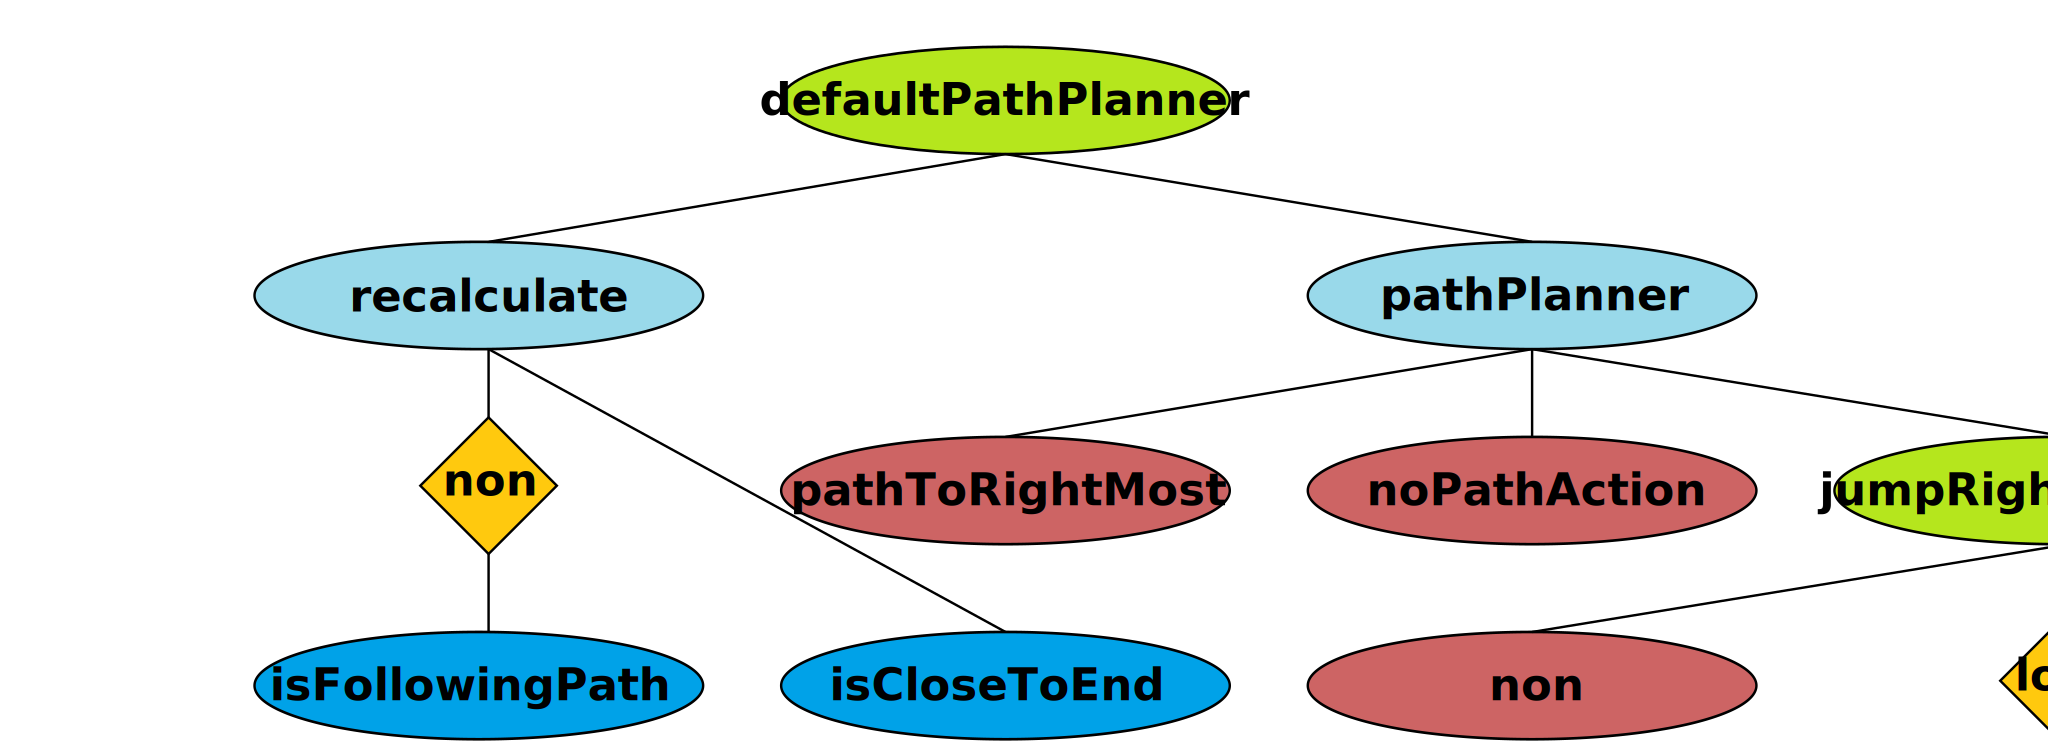
\includegraphics[scale=0.073]{images/lastButOne2}
	\caption{First sub-tree for path planning. It calculates, if needed, the path
	to the rightmost position available.}
	\label{fig:lastButOne}
	\end{center}
\end{figure}

Its root is a sequence node with two children. 
The first one (\textit{Recalculate}) decides if the default path 
%has to be calculated. That can happen when no one is being 
%followed or when a path has been set but it is about to be finished,
%so it is time to calculate the next one. Notice that the former 
has to be calculated. That can happen when no item is being targeted,
or when a path has been set but is about to be finished. Note that the former
reason allows potential paths requested by the reactive part not 
to be overwritten by the default planner. 

The second child (\textit{Path Planner}), executed if the one before 
is successful, calculates the path to the right most position in the 
map (which is the direction to follow to the level end). In the unusual 
case of not finding a path, Mario enters an emergency situation: in order 
to keep moving, a default forward jump is executed.

Finally, the second sub-tree checks if a path
has been set and, if that is the case, executes the action in charge of following the path.

%Said at the beginning, no image.
%The second sub-tree (figure~\ref{fig:lastSubTree}) of the path planning structure, 
%and hence the last child of the \texttt{rootSelector}, is very simple. 
%It checks if a path has been set and, if that is the case, 
%it executes the action in charge of following the path.

%\begin{figure} [ht]
%	\begin{center}
%	\includegraphics[scale=0.1]{images/lastSubTree}
%	\caption{Second sub-tree for path planning. Follows the current path if applicable.}
%	\label{fig:lastSubTree}
%	\end{center}
%\end{figure}

\subsection{Extensions to GE}

With the syntax described above, each \texttt{BehaviourBlock} becomes a
self-contained structure, and it makes sense to allow individuals to exchange
these between them. To this end, specific crossover points were encoded in the
grammar, bounding these blocks for exchange. This is a recent technique
\cite{ND06} in which a special grammar symbol
is used to label crossover points; the search algorithm then only
slices an individual according to these points. We extended this by using a
two-point crossover, effectively creating an operator much like sub-tree
crossover in GP \cite{Koz92}, but allowing the exchange of
different numbers of blocks between individuals. Without these markers, the
standard 1-point crossover as used in standard GE would provide more
exploration but less exploitation, and given the expensiveness of the fitness
function, a trade-off seemed to make sense.

Finally, an individual is allowed
to crossover with himself, thus creating a sub-tree swap operation;
this makes sense, as a mean to increase (or decrease) the priority of a
\texttt{BehaviourBlock}: the further to the left (right) within the
\texttt{rootSelector}, the bigger (smaller) the likelihood of execution of a
block.

\subsection{Generalisation Issues}

A difficulty with such a dynamic problem is that of generalisation performance.
In the Mario AI competition \cite{TKK09}, the off-line generated controllers
are tested in a series of randomly-generated maps; the difficulty of these maps
can be drastically different, ranging from surprisingly easy to virtually
impossible (for the same difficulty level). Taking this into account, three
approaches were tested to evolve BTs with GE:
\begin{itemize}
	%\item \textbf{Run5}: test each controller in a group of five
	%randomly generated sets of maps, which are never changed throughout the
	\item \textbf{Run5}: test each controller in five
	random sets of maps, which are never changed throughout the
	evolutionary cycle (and indeed are the same for all runs);
	\item \textbf{Change1}: only test one level, but change the random seed
	of that level at every generation (same set of seeds for each run),
	reevaluating the parent population with the new map only, thus
	allowing for more evolution cycle generations for the same amount
	of evaluations;
	\item \textbf{Run1}: always test in one ``typical'' level (same seed
	for all runs), assuming that the agent is presented with enough enemy
	and obstacle diversity to evolve good reactiveness routines, allowing
	for the biggest number of evolution cycle generations.
\end{itemize}

%%%%%%%%%%%%%%%%%%%%%%%%%%%%%%%%%%%%%%%%%%%%%%%%%%%%%%%%%%%%%%%%%%%%%%%%%%%%%%%
\section{Experiments}
%%%%%%%%%%%%%%%%%%%%%%%%%%%%%%%%%%%%%%%%%%%%%%%%%%%%%%%%%%%%%%%%%%%%%%%%%%%%%%%

\subsection{Setup}

The experimental parameters used are shown in Table \ref{tab:gesetup}. All
individuals in the initial generation were valid \cite{RA03}, and
a variation of tournament selection was used, which ensures that each
individual participates at least in one tournament event. Also, the mutation
rate was set such that, on average, one mutation event occurs per
individual (regardless of their size).

\begin{table}[ht]
	\begin{center}
	\caption{Experimental Setup}
	\label{tab:gesetup}
	\begin{tabular}{|c|l|r|}
		\hline
		&Population Size & 500\\
		&Evaluations     & 125000\\
		&Derivation-tree Depth Range (for initialisation) & 20\ldots30\\
		&Tail Ratio (for initialisation) & 50\%\\
		GE&Selection Tournament Size & 1\%\\
		&Elitism (for generational replacement) & 10\%\\
		&Marked 2-point Crossover Ratio & 50\%\\
		&Marked Swap Crossover Ratio & 50\%\\
		&Average Mutation Events per Individual & 1\\
		\hline
		\ Mario\ &Level Difficulties & 0\ldots4 \\
		&Level Types & 0 1 \\
		&Level Lengths & 320\\
		\hline
	\end{tabular}
	\end{center}
\end{table}

Each evaluation is comprised of 10 levels (5 difficulty settings, with two
types of map each). All three approaches (Run5, Change1 and Run1) were tested on
30 different runs, for statistical purposes. The individual fitness value, to be maximized, 
is a weighted sum of distance travelled and some other factors, like enemy kills and 
collected items.

%%At each generation, each individual is evaluated on 18 levels (9 difficulty
%%settings, with two types of map each). As the competition runs on unseen maps,
%%we had to ensure a level of generalisation for the evolved solutions. The ideal
%%approach would be to greatly increase the sample of levels available for
%%evaluation, but given that evaluation is a very expensive process (between two
%%and ten seconds per individual for 18 maps, on a $3.06$ GHz Intel Core 2 Duo
%%processor), a different solution had to be found.
%%
%%To this end, the sample of maps for evaluation is changed at each generation;
%%to avoid loosing information acquired from previous generations, the parent
%%population is reevaluated at each generation with the new maps, and each
%%individual's fitness is averaged between the previous scores and the new one.
%%Although the offspring fitness is based on the new available maps only, elitism
%%ensures that a percentage of the (potentially better generalised) solutions
%%from the parent population are kept for the next generation.
%
%At each generation, each individual is evaluated on 18 levels (9 difficulty
%settings on two level types). To enforce generalisation, the
%%set of maps for evaluation is changed at each generation; to avoid loosing
%%information acquired from previous generations, the parent population is
%set of maps for evaluation is changed at each generation; the parent population
%is re-evaluated with the new maps, and each individual's fitness is averaged
%between the previous scores and the new one. Although the offspring fitness is
%based on the new maps only, elitism ensures that a percentage of the
%(potentially more general) solutions from the parent population are kept for
%the next generation.

%A series of runs with different random seeds were executed in parallel in a
%small cluster. At the end of all runs, all best individuals were evaluated in
%600 unseen maps, and the best overall solution was submitted to the
%competition.
%
%%%%%%%%%%%%%%%%%%%%
\subsection{Results}

Fig.~\ref{fig:training} shows the mean best individual fitness, for all three
approaches, averaged across all runs. The graph shows that the Run1
approach was quite successful at optimising the controller behaviour, for the
map that it was tested on. The Run5 approach also shows improvement over time,
albeit at a lower rate. Finally, the Change1 approach seems quite noisy, which
is a clear indication of the extreme range of difficulty of maps generated with
different random seeds, even with the same difficulty setting.

\begin{figure}[ht]
	\begin{center}
	\includegraphics[width = .33\textwidth, angle=270]{images/mbi}
	\caption{Mean best individual score for all three approaches, averaged
	across 30 independent runs.}
	\label{fig:training}
	\end{center}
\end{figure}

A generalisation test was also devised, which consisted of 360 unseen levels
(20 different random seeds, each generating 9 difficulty levels, with two types
of map each). The best individual at every $5000$ evaluations was tested, and
the averaged results across all runs are shown in Fig.~\ref{fig:generalisation}.

\begin{figure}[ht]
	\begin{center}
	\includegraphics[width = .33\textwidth, angle=270]{images/mbg}
	\caption{Generalisation score of the best individual every $50000$
	evaluations,  for all three approaches, averaged across 30 independent
	runs.}
	\label{fig:generalisation}
	\end{center}
\end{figure}

The results show interesting differences between the three approaches. The Run1
approach starts by improving its score, but very rapidly worsens it.
This is a clear sign of over-fitting: the evolved controllers were tested in a
single map, and a comparison with Fig.~\ref{fig:training} shows that,
despite an improving training score, the generalisation score keeps worsening.

The Run5 approach shows the most stable results. The generalisation score
improves over time, albeit slowly; with a limited number of maps
to train on, the evolved controllers quickly converge to an overall
\textit{average} behaviour, as seen in Fig.~\ref{fig:training}, and with
evolution stagnated (roughly after $80000$ evaluations), there is little or no
generalisation improvement.

Finally, the results of the Change1 approach are the most interesting. These
highlight once again the variety of scores that can be achieved with
differently seeded maps. Although the generalisation score is very irregular,
there is an overall trend to improve it across time, and the scores achieved
are the best of all three approaches.

%The four \texttt{BehaviourBlocks} of the best BT generated, are shown in
%%Table \ref{tab:final}. The first block is composed of two
%Fig.~\ref{fig:final}. The first block is composed of two
%conditions, followed by a sequence of actions (not shown). The conditions check
%for any jumpable platform on the right, and if there are no obstacles in the
%way. The sequence of actions is composed of 15 actions and sub-trees, that make
%Mario jump, run to the right and fire.
%%The best overall individual, sent to the competition, was composed of a
%%\texttt{rootSelector} with four \texttt{BehaviourBlock}s, and is shown in
%%Fig.~\ref{fig:final}.

%The next block contains a very relevant sub-tree: \texttt{AvoidRightTrap}. It
%is used to escape from dead-ends, such as shown in Fig.~\ref{fig:deadEnd}; this
%is one of the hardest obstacles encountered in a level.

%The third block checks if Mario is stuck between a hole and an enemy, and if so
%executes a sequence of actions for jumping, shooting and running.
%Finally, the last (default) block contains the sequence \texttt{RunRightSafe},
%\texttt{Fire} and \texttt{RunRightSafe}, instructing Mario to run to the right
%while shooting, and to avoid enemies and holes by jumping.

%\begin{figure} [ht]
%	\begin{center}
%	\includegraphics[scale=0.11]{images/treeBlocks}
%	\caption{Behaviour tree blocks of the final individual.}
%	\label{fig:final}
%	\end{center}
%\end{figure}

%\begin{figure} [ht]
%	\begin{center}
%	\includegraphics[scale=0.8]{images/deadEnd}
%	\caption{Level dead end. Mario has to come back and find another way.}
%	\label{fig:deadEnd}
%	\end{center}
%\end{figure}

%%%%%%%%%%%%%%%%%%%%%%%%%%%%%%%%%%%%%%%%%%%%%%%%%%%%%%%%%%%%%%%%%%%%%%%%%%%%%%%
\section{Conclusions}
%%%%%%%%%%%%%%%%%%%%%%%%%%%%%%%%%%%%%%%%%%%%%%%%%%%%%%%%%%%%%%%%%%%%%%%%%%%%%%%

This paper presented an extension of previous work \cite{PNO11}, evolving
Behaviour Trees for the Mario AI Benchmark. The A* algorithm was applied in a
dynamic manner, constantly providing path planning routines that were combined
with reactive routines in BTs; these trees were then evolved using Grammatical
Evolution.

The combination of a Genetic Programming type algorithm with BTs provided a
flexible approach. The resulting solutions are human readable, and
thus easy to analyse and fine-tune, which aims at one of the main concerns
of the game industry regarding evolutionary approaches, as stated early in 
section~\ref{sec:intro}. Also, the use of a grammar allows full
syntactic control of the resulting BTs, providing full control of their
breadth, depth, and overall complexity. Finally, the
combination of a carefully designed syntax with specific crossover locations
allows the definition and exchange of meaningful behaviour blocks, accelerating
the evolutionary process.

One of the potential drawbacks of using a stochastic algorithm is the need for
an evolutionary process, making online learning difficult (and sometimes
impossible). By applying the A* algorithm in a dynamic manner, however, the
evolved behaviours remain adaptive, particularly in what concerns navigation.

The experiments and results presented are relevant in many aspects. They
highlight the dynamic nature of game environments; with such a multitude of
possible environments and situations to face (and the disparity of possible
fitness scores), there is a real risk of over-fitting to specific game
situations, and experimental design is of the utmost importance. Of all the
approaches presented, the one with the best results reevaluated all individuals
at each generation in a new set of unseen maps; this resulted in a very noisy
fitness landscape, but in the end provided the best generalisation results.

Future work will aim to improve these results. There exists a wide body of research work
dealing with the problem of over-fitting, and techniques such as using training
and generalisation sets for early stopping of the evolutionary process
\cite{Pre97}, or sliding windows of training cases \cite{WAW07}, should provide
better generalisation scores. It will also be interesting to compare the performance of
the GE algorithm with similar ones, as for instance a strongly typed tree-based 
Genetic Programming approach.

Finally, a controller combining all the techniques described in this paper will
be submitted to the Mario AI Benchmark competition \cite{JSR10}, allowing its
comparison with other existing approaches.

\section*{Acknowledgments}
This research is based upon works supported by the Science Foundation Ireland
under Grant No. 08/IN.1/I1868.


%\bibliographystyle{splncs03}
\begin{thebibliography}{11}
	\bibitem{Ake78}
	Binary Decision Diagrams.
	IEEE Transactions on Computers, C-27(6), pp.~509–-516. (1987)
	\bibitem{Ang97}
	P.~Angeline:
	Subtree Crossover: Building Block Engine or Macromutation?.
	In: Genetic Programming 1997, Proceedings.
	Morgan Kaufmann (1997)
	pp.~9--17
	\bibitem{BT98}
	S.~Bandi, D.~Thalmann:
	Space discretization for efficient human navigation.
	In: Computer Graphics Forum, Vol.~17, Issue 3, September 1998
	pp.~195--206
	\bibitem{Bir99}
	K.~Birdwell:
	The CABAL: Valve's Design Processing for Creating Half Life.
	In: Game Developer 6 (12) (1999)
	pp.~40--50
	\bibitem{BC10}
	Bojarski, S.;   Congdon, C.B.;
	REALM: A rule-based evolutionary computation agent that learns to play Mario.
	In: 2010 IEEE Symposium on Computational Intelligence and Games (CIG) (2010).
	pp.~83--90
	\bibitem{CBP99}
	Cavazza, M.; Bandi, S.; and Palmer, I.:
	“Situated AI” in Video Games: Integrating NLP, Path Planning, 
	and 3D Animation.
	In:  Papers from the AAAI 1999 Spring Symposium on Artificial 
	Intelligence and Computer Games (1999)
	Technical Report SS-99-02.
	pp.~6--12
	\bibitem{CDC10}
	A.~Champandard, M.~Dawe and D.~H.~Cerpa:
	Behavior Trees: Three Ways of Cultivating Strong AI.
	In: Game Developers Conference, Audio Lecture. (2010)
	\bibitem{Cha07}
	A.~Champandard:
	Behavior Trees for Next-Gen Game AI.
	In: Game Developers Conference, Audio Lecture. (2007)
	\bibitem{CH07}
	R.~Colvin and I.~J.~Hayes:
	A Semantics for Behavior Trees.
	ARC Centre for Complex Systems, tech.~report ACCS-TR-07-01. (2007)
	\bibitem{Gol89}
	D.~E.~Goldberg:
	Genetic Algorithms in Search, Optimization and Machine Learning.
	Addison Wesley (1989)
	\bibitem{Isl05}
	D.~Isla:
	Managing Complexity in the Halo 2 AI System.
	In: Game Developers Conference, Proceedings. (2005)
	\bibitem{JSR10}
	J.~Togelius, S.~Karakovskiy and R.~Baumgarten:
	The 2009 Mario AI Competition.
	In: IEEE Congress on Evolutionary Computation, Proceedings.
	IEEE Press (2010)
	pp.~1--8
	\bibitem{Koz92}
	J.~R.~Koza:
	Genetic Programming: On the Programming of Computers by Means of Natural Selection.
	MIT Press (1992)
	\bibitem{LBC10}
	C.~Lim, R.~Baumgarten and S.~Colton:
	Evolving Behaviour Trees for the Commercial Game DEFCON.
	In: Applications of Evolutionary Computation, EvoApplications 2010, Proceedings. (2010)
	\bibitem{MNW10}
	R.~I.~McKay, X.~H.~Nguyen, P.~A.~Whigham, Y.~Shan and M.~O'Neill:
	Grammar-Based Genetic Programming - A Survey.
	Genetic Programming and Evolvable Machines, 11(3-4). (2010)
	pp.~365--396
	\bibitem{MF03}
	J.~Meyer, D.~Filliat:
	Map-based navigation in mobile robots: II. A review of map-learning 
	and path-planning strategies.
	Cognitive Systems Research, 4(4). (2003)
	pp.~283--317
	\bibitem{Mch07}
	L.~McHugh:
	Three Approaches to Behavior Tree AI.
	In: Game Developers Conference, Proceedings. (2007)
	\bibitem{MMM10}
	A.~M.~Mora, R.~Montoya, J.~J.~Merelo, P.~G.~S\'anchez, P.~A.~Castillo,
	J.~L.~J.~Laredo, A.~I.~Mart\'inez and A.~Espacia:
	Evolving Bot AI in Unreal.
	In: Applications of Evolutionary Computation, EvoApplications 2010, Proceedings.
	Springer Verlag. (2010)
	pp.~171--180
	\bibitem{MS04}
	M.~Mateas and A.~Stern:
	Managing Intermixing Behavior Hierarchies.
	In: Game Developers Conference, Proceedings. (2004)
	\bibitem{ND06}
	M.~Nicolau and I.~Dempsey:
	Introducing Grammar Based Extensions for Grammatical Evolution.
	In: IEEE Congress on Evolutionary Computation, Proceedings.
	IEEE Press (2006)
	pp.~2663--2670
	\bibitem{Nil98}
	N.~J.~Nilsson:
	Artificial Intelligence, A New Synthesis.
	Morgan Kaufmann Publishers. (1998)
	\bibitem{NL04}
	S.~Nason and J.~Laird:
	Soar-RL: Integrating Reinforcement Learning with Soar.
	In: International Conference on Cognitive Modelling, Proceedings. (2004)
	\bibitem{OR03}
	M.~O'Neill and C.~Ryan:
	Grammatical Evolution: Evolutionary Automatic Programming in a Arbitrary Language.
	Kluwer Academic Publishers (2003)
	\bibitem{PNO11}
	D.~Perez and M.~Nicolau and M.~O'Neill and A.~Brabazon.
	Evolving Behavior Trees for the Mario AI Competition Using Grammatical Evolution.
	In Applications of Evolutionary Computation, EvoApplications 2011, Proceedings.
	Springer Verlag. (2011)
	pp.~121--130
	\bibitem{Pre97}
	L.~Prechelt.
	Early Stopping - But When?.
	In Neural Networks: Tricks of the Trade, Proceedings.
	Springer Verlag. (1997)
	pp.~55--69
	\bibitem{Pri09}
	S.~Priesterjahn:
	Imitation-Based Evolution of Artificial Game Players.
	ACM SIGEVOlution, 2(4). (2009)
	pp.~2--13
	\bibitem{RA03}
	C.~Ryan and R.~M.~A.~Azad:
	Sensible initialisation in grammatical evolution.
	In: Barry, A.M. (ed.) {GECCO 2003}: Proceedings of the Bird of a Feather Workshops.
	AAAI (2003)
	pp.~142--145.
	\bibitem{SOG03}
	K.~Sastry, U.~O'Reilly, D.~E.~Goldberg and D.~Hill:
	Building Block Supply in Genetic Programming.
	Genetic Programming Theory and Practice, Chapter 4.
	Kluwer Publishers (2003)
	pp.~137--154
	\bibitem{TBS04}
	C.~Thurau, C.~Bauckhauge and G.~Sagerer:
	Combining Self Organizing Maps and Multiplayer Perceptrons to Learn
	Bot-Behavior for a Comercial Game.
	In: GAME-ON'03 Conference, Proceedings. (2003)
	\bibitem{TKB10}
	J.~Togelius, S.~Karakovskiy and R.~Baumgarten:
	The 2009 Mario AI Competition.
	In: IEEE Congress on Evolutionary Computation, Proceedings.
	IEEE Press (2010)
	\bibitem{TKK09}
	J.~Togelius, S.~Karakovskiy, J.~Koutnik and J.~Schmidhuber:
	Super Mario Evolution.
	In: IEEE Symposium on Computational Intelligence and Games, Proceedings.
	IEEE Press (2009)
	\bibitem{WAW07}
	S.~Winkler, M.~Affenzeller, and S.~Wagner:
	Selection Pressure Driven Sliding Window Behavior in Genetic
	Programming Based Structure Identification.
	In: EUROCAST'07 Conference, Proceedings.
	Springer-Verlag (2007)
	pp.~788--795
\end{thebibliography}

\end{document}

